\chapter{生物地球化学循环}\label{ch:b2:biogeochemical-cycles}

1958 年 3 月，年轻的化学家查尔斯·基林在
夏威夷莫纳罗亚山的北坡打开了一台红外线气体分析仪，
那里高出太平洋 3.5 千米，空气
混合得再好不过。他原以为会测到一个常数；
不到一年，他得到的却是一条锯齿状曲线——二氧化碳每年冬季上升、
夏季下降，这是北半球森林
一呼一吸的结果——数年之后，锯齿之下出现了一条斜线，
此后一直在上升，至今未停。\omterm{prop:b2:biogeochemical-cycles:carbon}{基林曲线}
是从外部看到的生物圈的呼吸，其上叠加了一张
体温记录图。本章讨论曲线所记录的循环：
生物体中碳、氮、磷和硫的储存位置，
它们在\omterm{def:b2:biogeochemical-cycles:reservoir}{储库}之间的转移速度，以及决定这些速度的因素——
其中多数是
\cref{ch:b2:microbial-metabolism}中的代谢过程——以及人类这一物种
两百年来对每个循环所造成的影响。

\section{储库、通量与停留时间}

\begin{definition}[储库、通量与停留时间]\label{def:b2:biogeochemical-cycles:reservoir}
\index{储库}\index{通量}\index{停留时间}\index{稳态}\index{生物地球化学循环}
\emph{生物地球化学循环}是元素在
\emph{储库}（大气、海洋、土壤、活
生物量、岩石）之间的迁移，由\emph{通量}实现，通量以每年的质量计。
质量为 $M$、总流出量为 $F$ 的储库具有\emph{停留
时间}$\tau = M/F$，即原子在其中停留的平均时间；在
\emph{稳态}下，流入量等于流出量，$M$ 为常数。各
循环通过生命的化学计量相互耦合——海洋浮游生物的
\emph{雷德菲尔德比}为 $\mathrm{C:N:P} =
106:16:1$（按原子数计），因此最稀缺元素的供应
决定了其他所有元素被吸收的速率。
\end{definition}

\begin{theorem}[单箱模型]\label{thm:b2:biogeochemical-cycles:box}
\index{箱式模型}\index{弛豫时间}
若\omterm{def:b2:biogeochemical-cycles:reservoir}{储库}以正比于其所含量的速率流失物质，
即 $F_{\text{出}} = M/\tau$，并接收恒定的
流入量 $F_{\text{入}}$，则
\[
\frac{\mathrm{d}M}{\mathrm{d}t} = F_{\text{入}} - \frac{M}{\tau},
\qquad
M(t) = M^{*} + (M_0 - M^{*})\,e^{-t/\tau}, \qquad M^{*} = F_{\text{入}}\tau :
\]
\omterm{def:b2:biogeochemical-cycles:reservoir}{储库}弛豫到与其输入成正比的\omterm{def:b2:biogeochemical-cycles:reservoir}{稳态}，
以\omterm{def:b2:biogeochemical-cycles:reservoir}{停留时间}为时间常数。输入的阶跃式增加
会按比例抬高\omterm{def:b2:biogeochemical-cycles:reservoir}{稳态}，\omterm{def:b2:biogeochemical-cycles:reservoir}{储库}在
几个 $\tau$ 内跟上：\omterm{def:b2:biogeochemical-cycles:reservoir}{停留时间}为数天的池，
如大气中的氨、春季湖泊中的硝酸盐，其含量紧随
来源而变化；\omterm{def:b2:biogeochemical-cycles:reservoir}{停留时间}长达数世纪的池（深海碳、
土壤有机质）则对其加以累积，而慢速池中的
扰动比引起它的那次扰动持续更久。
\end{theorem}
\begin{proof}
方程为常系数线性方程：\omterm{def:b2:biogeochemical-cycles:reservoir}{稳态}
$M^{*}$ 使右端为零，偏差 $m = M - M^{*}$
满足 $\dot m = -m/\tau$，故 $m = m_0 e^{-t/\tau}$。若\omterm{def:b2:biogeochemical-cycles:reservoir}{储库}
有多条流出途径，则 $\tau$ 由它们之和决定，$1/\tau = \sum_i
1/\tau_i$：最快的库起主导作用。
\end{proof}

\section{碳循环}

\begin{proposition}[碳收支]\label{prop:b2:biogeochemical-cycles:carbon}
\index{碳循环}\index{大气分数}\index{碳汇}\index{基林曲线}
以吉吨碳为单位（\unit{GtC}，$10^{12}$~kg），主要\omterm{def:b2:biogeochemical-cycles:reservoir}{储库}有
大气（2020 年代约 880，
工业化前约 590）、陆地植物（450）、土壤（1700）、表层
海洋（900）、深海（\num{37000}）和沉积岩
（\num{e8}）；化石燃料是后者中工业所能
触及的部分，约 \num{5000}。自然\omterm{def:b2:biogeochemical-cycles:reservoir}{通量}很大，
且近乎平衡：陆地光合作用每年固定约 120，
由呼吸与分解作用归还；海洋
表层与大气之间每个方向约交换 80。人为\omterm{def:b2:biogeochemical-cycles:reservoir}{通量}
相比之下很小：来自化石燃料的每年约 10，
来自毁林的约 1，但它是单向的，大气保留了其中
\emph{约 \qty{45}{\%}}（即\emph{\omterm{prop:b2:biogeochemical-cycles:carbon}{大气分数}}），
海洋吸收了四分之一，陆地受额外 $\mathrm{CO_2}$ 施肥，
吸收了其余部分。大气中百万分之一的 $\mathrm{CO_2}$ 相当于
\qty{2.13}{GtC}；浓度从 280 上升到 \num{315}~ppm，
时段为 1750 年至 1958 年，又从 315 升至 \num{420} 以上，时段为
1958 年至 2020 年代，目前每年增加 \qty{2.5}{ppm}。空气中
$\mathrm{CO_2}$ 分子的\omterm{def:b2:biogeochemical-cycles:reservoir}{停留时间}为 $880/200 \approx 4$ 年，
较短；而\emph{超出量}的寿命，取决于向深海的缓慢混合
和更慢的岩石风化，
为数世纪至数千年——今天所排放的物质中，五分之一将
在一万年后仍留在大气中。
\end{proposition}
\begin{proof}[证据]
三个特征表明，新增的碳来自化石燃料。其
同位素方面，化石碳不含 $\mathrm{{}^{14}C}$（它早已
在数百万年前衰变殆尽），且 $\mathrm{{}^{13}C}$ 含量偏低，与一切植物碳相同，
而大气中这两种同位素都在减少——这就是
苏伊斯效应，自 1950 年代以来在树轮中测得。其氧方面：大气中的
$\mathrm{O_2}$ 同步下降，依据
燃烧的化学计量，这已由基林之子在 1990 年代证实，而火山
或海洋来源则不会产生。其收支核算：
售出的煤、石油和天然气（折算为碳）之和，
超过大气增量的两倍，缺失的一半
见于海洋中溶解无机碳的上升与 pH 的下降，以及
陆地\omterm{prop:b2:biogeochemical-cycles:carbon}{碳汇}。季节性锯齿在阿拉斯加的巴罗
比在莫纳罗亚山更大，而在南极点几乎不见，它是
北方森林夏季吸收、冬季释放的结果——
对生物圈呼吸的直接测量。
\end{proof}

\begin{omfigure}
\begin{tikzpicture}
\begin{axis}[
  width=0.9\linewidth, height=6cm,
  axis x line=bottom, axis y line=left,
  xmin=1955, xmax=2026, ymin=300, ymax=430,
  xlabel={年}, ylabel={$\mathrm{CO_2}$（ppm），莫纳罗亚山年平均值},
  xlabel style={font=\small, at={(axis description cs:0.5,-0.13)}, anchor=north},
  ylabel style={font=\small},
  tick label style={font=\small}, xtick={1960,1970,1980,1990,2000,2010,2020}, ytick={300,325,350,375,400,425},
  scaled x ticks=false, x tick label style={/pgf/number format/1000 sep=},
  clip=false,
]
\addplot[very thick, omDef, mark=*, mark size=1pt] coordinates {
(1959,316.0) (1962,318.5) (1965,320.0) (1968,323.0) (1971,326.3) (1974,330.2) (1977,333.8) (1980,338.8) (1983,342.8) (1986,347.2) (1989,353.1) (1992,356.4) (1995,360.8) (1998,366.7) (2001,371.1) (2004,377.5) (2007,383.8) (2010,389.9) (2013,396.5) (2016,404.2) (2019,411.4) (2022,418.5) (2024,424.6)};
\node[font=\scriptsize, anchor=north west, align=left] at (axis cs:1958,425) {1960 年代：\qty{+0.9}{ppm/yr}\\2010 年代：\qty{+2.4}{ppm/yr}};
\node[font=\scriptsize, anchor=west, align=left] at (axis cs:1990,320) {工业化前水平：\qty{280}{ppm}；\\每年都有 $\pm\qty{3}{ppm}$ 的锯齿叠在这条线上};
\end{axis}
\end{tikzpicture}

{\small \omterm{prop:b2:biogeochemical-cycles:carbon}{基林曲线}：大气中二氧化碳的年平均含量，
自 1959 年起在莫纳罗亚火山测得。斜率几乎增至三倍；
其上的季节性锯齿（本比例下未画出）是
北半球夏季光合作用的结果。}
\end{omfigure}

\begin{omfigure}
\begin{tikzpicture}[every node/.style={font=\scriptsize}, >=stealth, box/.style={draw, rounded corners, minimum width=2.2cm, minimum height=0.9cm, align=center, fill=#1}]
  \node[box=omDef!15] (atm) at (0,3) {大气 \\880};
  \node[box=omThm!15] (veg) at (-4.4,0.6) {陆地植物 450\\土壤 1700};
  \node[box=omProp!15] (surf) at (4.4,0.6) {表层海洋 \\900};
  \node[box=omProp!25] (deep) at (4.4,-1.6) {深海 \\37\,000};
  \node[box=gray!20] (rock) at (0,-1.6) {岩石与化石燃料 \\$10^{8}$；可开采 $\sim 5000$};
  \draw[->, thick] ([xshift=-2mm]atm.south west) -- node[above left, pos=0.45] {120 光合作用} ([xshift=-4mm]veg.north);
  \draw[->, thick] ([xshift=5mm]veg.north) -- ([xshift=-2mm]atm.south); \node[anchor=north east] at (-0.4,1.5) {119 呼吸、火灾};
  \draw[->, thick] ([xshift=2mm]atm.south east) -- node[above right, pos=0.45] {80 溶解} ([xshift=4mm]surf.north);
  \draw[->, thick] ([xshift=-5mm]surf.north) -- ([xshift=2mm]atm.south); \node[anchor=north west] at (0.4,1.5) {78 释放};
  \draw[<->, thick] (surf) -- node[right] {$\sim 100$ 混合、下沉} (deep);
  \draw[->, very thick, omExo!80!black] (rock.north) -- node[left, align=right, pos=0.4] {10 化石燃料 \\ + 1 土地利用} (atm.south);
  \node[align=left, anchor=west] at (7.0,3.2) {通量单位：\unit{GtC/yr}，\\ 库存单位：\unit{GtC}\\[2pt] 排放的 11 中：\\ 5 留在大气中，\\ 3 进入陆地，\\ 3 进入海洋};
\end{tikzpicture}

{\small \omterm{prop:b2:biogeochemical-cycles:carbon}{碳循环}的粗略数值。天然交换
量是人为\omterm{def:b2:biogeochemical-cycles:reservoir}{通量}的十倍，但二者几乎相互抵消；人为
\omterm{def:b2:biogeochemical-cycles:reservoir}{通量}则不然。}
\end{omfigure}

\begin{omfigure}
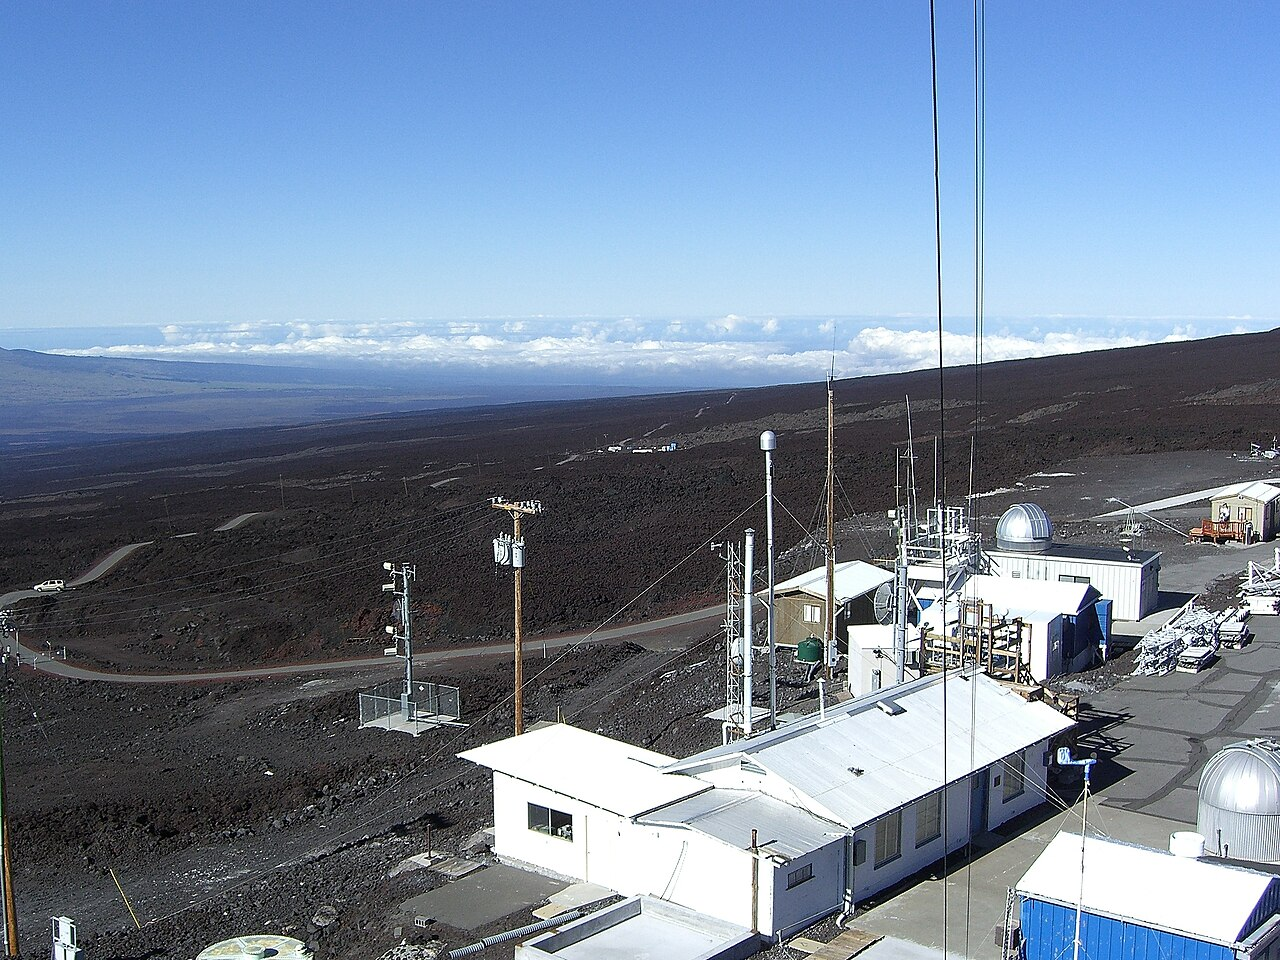
\includegraphics[width=0.56\linewidth]{images/book4/mauna-loa.jpg}\hspace{0.03\linewidth}
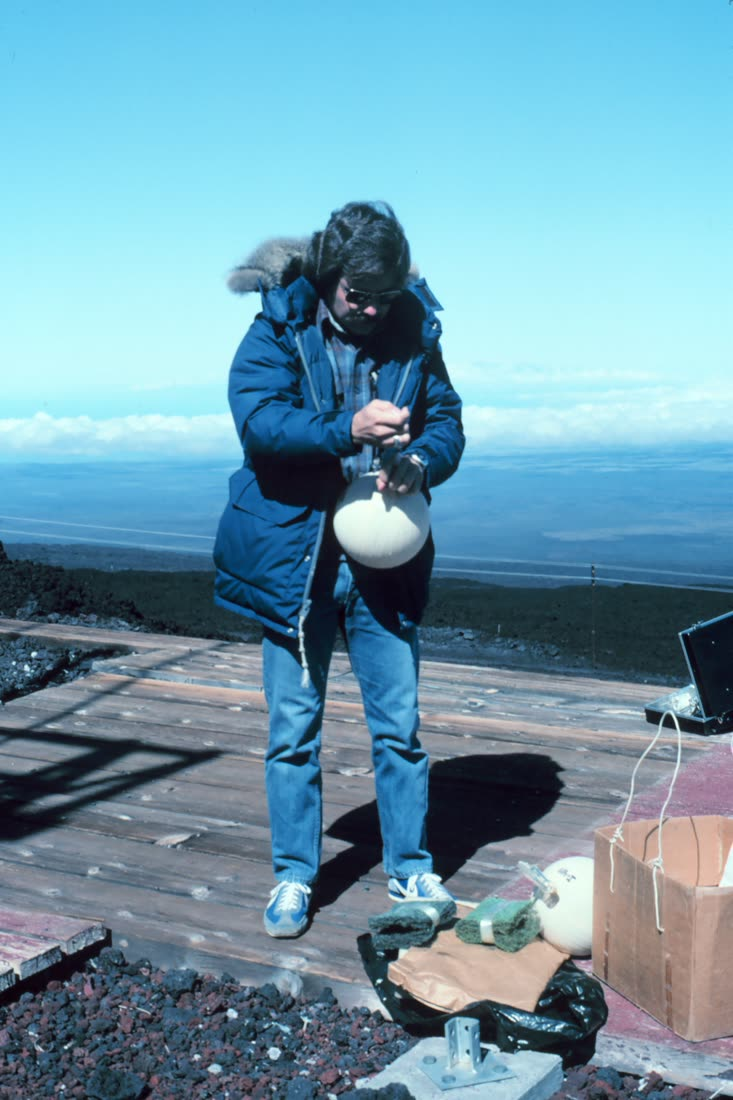
\includegraphics[width=0.33\linewidth]{images/book4/keeling-flask.jpg}

{\small 曲线的绘制地点。左：莫纳罗亚火山北侧的
观测站，海拔 \qty{3400}{m}，位于信风逆温层之上，
该逆温层使岛上自身的空气留在其下。右：正在
采集样本的烧瓶（摄于 1982 年）；此类烧瓶在加利福尼亚分析，
用以核对连续分析仪，并在
从阿拉斯加到南极的各站点灌装。}
\end{omfigure}

\section{氮循环}

\begin{proposition}[氮循环]\label{prop:b2:biogeochemical-cycles:nitrogen}
\index{氮循环}\index{固氮}\index{硝化作用}\index{反硝化作用}\index{哈伯–博施法}\index{厌氧氨氧化}
氮储量丰富——空气中含有 $4\times 10^{9}$~Tg 的
$\mathrm{N_2}$——但氮却稀缺，因为 $\mathrm{N_2}$ 的三键仅由
两种过程打开：闪电（每年数 Tg）和
\emph{生物\omterm{prop:b2:biogeochemical-cycles:nitrogen}{固氮}}，由带有\omterm{prop:b2:biogeochemical-cycles:nitrogen}{固氮}酶的\omterm{def:b2:unicellular-diversity:prokaryote}{原核生物}完成，
陆地每年约 100 Tg、海洋约 100 Tg，每固定一个
$\mathrm{N_2}$ 需耗 16 个 ATP。固定态氮随后在
微生物驱动的氧化还原阶梯上流转（见\cref{ch:b2:microbial-metabolism}）：
\emph{氨化作用}使死亡有机物转化为 $\mathrm{NH_4^{+}}$；
\emph{\omterm{prop:b2:microbial-metabolism:lithotrophy}{硝化作用}}使 $\mathrm{NH_4^{+}}$ 转化为 $\mathrm{NO_2^{-}}$ 和 $\mathrm{NO_3^{-}}$，由
好氧化能自养生物完成；植物吸收 $\mathrm{NH_4^{+}}$ 或 $\mathrm{NO_3^{-}}$，
并将其还原回胺；在无氧条件下，
\emph{\omterm{def:b2:microbial-metabolism:anaerobic}{反硝化作用}}使 $\mathrm{NO_3^{-}}$ 转化为 $\mathrm{N_2}$（伴有 $\mathrm{N_2O}$ 作为
泄漏）；以及\emph{\omterm{prop:b2:biogeochemical-cycles:nitrogen}{厌氧氨氧化}}，即在无氧条件下以
亚硝酸盐氧化铵生成 $\mathrm{N_2}$，两者合计回到大气的量
与\omterm{prop:b2:biogeochemical-cycles:nitrogen}{固氮}所固定的量大致相当。氮原子在
生物圈中的\omterm{def:b2:biogeochemical-cycles:reservoir}{停留时间}为数百年；在大气中，约为 $4\times
10^{9}/400 \approx 10^{7}$ 年。自 1913 年起，\emph{哈伯–博施}法
已通过工业方式\omterm{prop:b2:biogeochemical-cycles:nitrogen}{固氮}，如今每年约 120 Tg，
栽培豆科植物与化石燃料燃烧又分别增加 60 和 30：
人类活动固定的氮量与一切自然过程之和相当，
并养活了现有人口的一半。
\end{proposition}

\begin{omfigure}
\begin{tikzpicture}[every node/.style={font=\scriptsize}, >=stealth, box/.style={draw, rounded corners, minimum width=1.9cm, minimum height=0.8cm, align=center, fill=#1}]
  \node[box=omDef!15] (n2) at (0,3.4) {空气中的 $\mathrm{N_2}$\\$4\times 10^{9}$ Tg};
  \node[box=omThm!15] (org) at (-4.6,1.0) {有机氮 \\植物、土壤、海洋};
  \node[box=omProp!15] (nh4) at (-2.2,-0.8) {$\mathrm{NH_4^{+}}$};
  \node[box=omProp!15] (no2) at (2.2,-0.8) {$\mathrm{NO_2^{-}}$};
  \node[box=omProp!15] (no3) at (4.6,1.0) {$\mathrm{NO_3^{-}}$};
  \draw[->, thick] (n2) -- node[above left, align=right] {固氮 \\固氮酶，200\\哈伯–博施 120} (org);
  \draw[->, thick] (org.south) -- node[below left] {氨化作用} (nh4.north);
  \draw[->, thick] (nh4) -- node[below] {硝化作用} (no2);
  \draw[->, thick] (no2) -- node[below right] {硝化作用} (no3);
  \draw[->, thick] (no3) to[bend left=18] node[above, pos=0.72] {同化} (org);
  \draw[->, thick, omExo!80!black] (no3) -- node[above right, align=left] {反硝化作用 \\（无氧），$\mathrm{N_2O}$ 泄漏} (n2);
  \draw[->, thick, omExo!80!black] (no2) -- node[right, pos=0.55, align=left] {厌氧氨氧化 \\（与 $\mathrm{NH_4^{+}}$）} (n2);
  \node[anchor=north, align=center] at (0,-1.5) {通量单位为 Tg N/年；除同化与氨化作用外，每一步均由原核生物完成};
\end{tikzpicture}

{\small 作为氧化还原阶梯的\omterm{prop:b2:biogeochemical-cycles:nitrogen}{氮循环}（植物既同化铵，
也同化硝酸盐）。\omterm{prop:b2:biogeochemical-cycles:nitrogen}{固氮}与\omterm{def:b2:microbial-metabolism:anaerobic}{反硝化作用}是通往大气的两扇
门，二者都由微生物完成；工业这扇门
如今与天然的那扇门相当。}
\end{omfigure}

\begin{proof}[证据]
新罕布什尔州哈伯德布鲁克实验林：1965 年，一整个
集水区被砍伐殆尽，并用除草剂使其保持裸露，
而相邻的一个集水区则保持原状，两者的溪流
各自被测量并分析了数年。被剥离的集水区
流失硝酸盐的速率是对照的 60 倍——土壤的
全部氮储备因不再被植物吸收，
被硝化并冲刷流失，同时带走钙与钾，并使溪水酸化。
该实验揭示了完整森林中\omterm{prop:b2:biogeochemical-cycles:nitrogen}{氮循环}的紧密性（
每公顷每年仅损失数千克氮，而循环量则达数百
千克），以及何物打破了这一循环。
\end{proof}

\section{磷与硫}

\begin{proposition}[两个无快速气相的循环]\label{prop:b2:biogeochemical-cycles:ps}
\index{磷循环}\index{硫循环}\index{富营养化}\index{二甲基硫醚}
\emph{磷}没有气态形式。磷通过
岩石中磷灰石的风化进入生态系统，整个陆地表面每年约 20 Tg，
并在土壤与湖泊中被多次循环利用——
湖泊表层水中的磷酸根离子在
数小时内即被吸收，随后进入沉积物，在其中停留
$10^{8}$ 年，即一个岩石循环的时长。因此，生命节约用磷，
且受磷限制：磷在海洋中的\omterm{def:b2:biogeochemical-cycles:reservoir}{停留时间}约为
\num{20000} 年，深海的磷酸盐经由上涌带回表层，
决定了海洋的生产力。如今，采矿向农田输入的磷
量与风化释放的量大致相当，其径流进入
湖泊后引发\emph{\omterm{prop:b2:biogeochemical-cycles:ps}{富营养化}}：藻华、其腐烂、
氧气的消耗，以及鱼类死亡——施林德勒的
安大略省 1970 年代进行的全湖实验中，一半湖泊
施用磷肥、另一半不施用，结果表明仅磷
即为诱因，并促成了洗涤剂中磷的去除。
\emph{硫}既有岩石循环（石膏、黄铁矿），又有
气相：火山与煤燃烧产生的 $\mathrm{SO_2}$，缺氧沉积物中的 $\mathrm{H_2S}$，
以及海洋浮游生物产生的\emph{\omterm{prop:b2:biogeochemical-cycles:ps}{二甲基硫醚}}，其
氧化产物为海洋上空的云提供凝结核。煤炭燃烧
在 20 世纪使进入大气的硫\omterm{def:b2:biogeochemical-cycles:reservoir}{通量}增为三倍，并
造成了欧洲与北美的酸雨；脱硫装置在数十年内
扭转了这一局面，大气中\omterm{prop:b2:biogeochemical-cycles:ps}{硫循环}的\omterm{def:b2:biogeochemical-cycles:reservoir}{停留时间}仅为
数天。
\end{proposition}

\begin{omfigure}
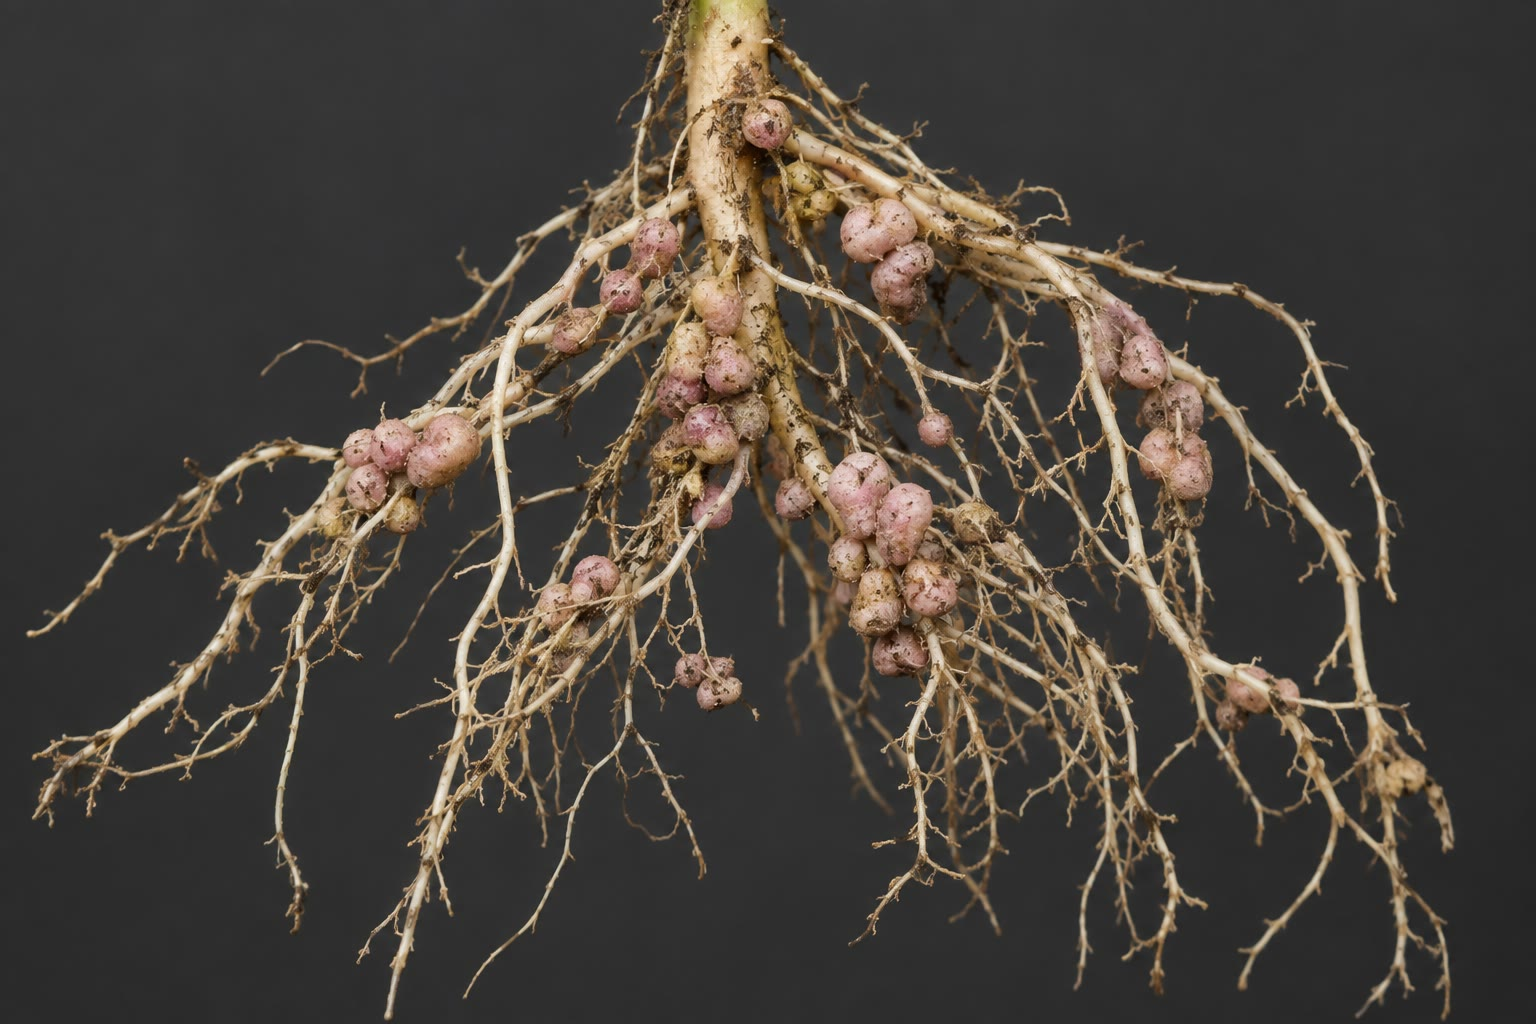
\includegraphics[width=0.44\linewidth]{images/book4/ai/b4-25-root-nodules.jpg}\hspace{0.04\linewidth}
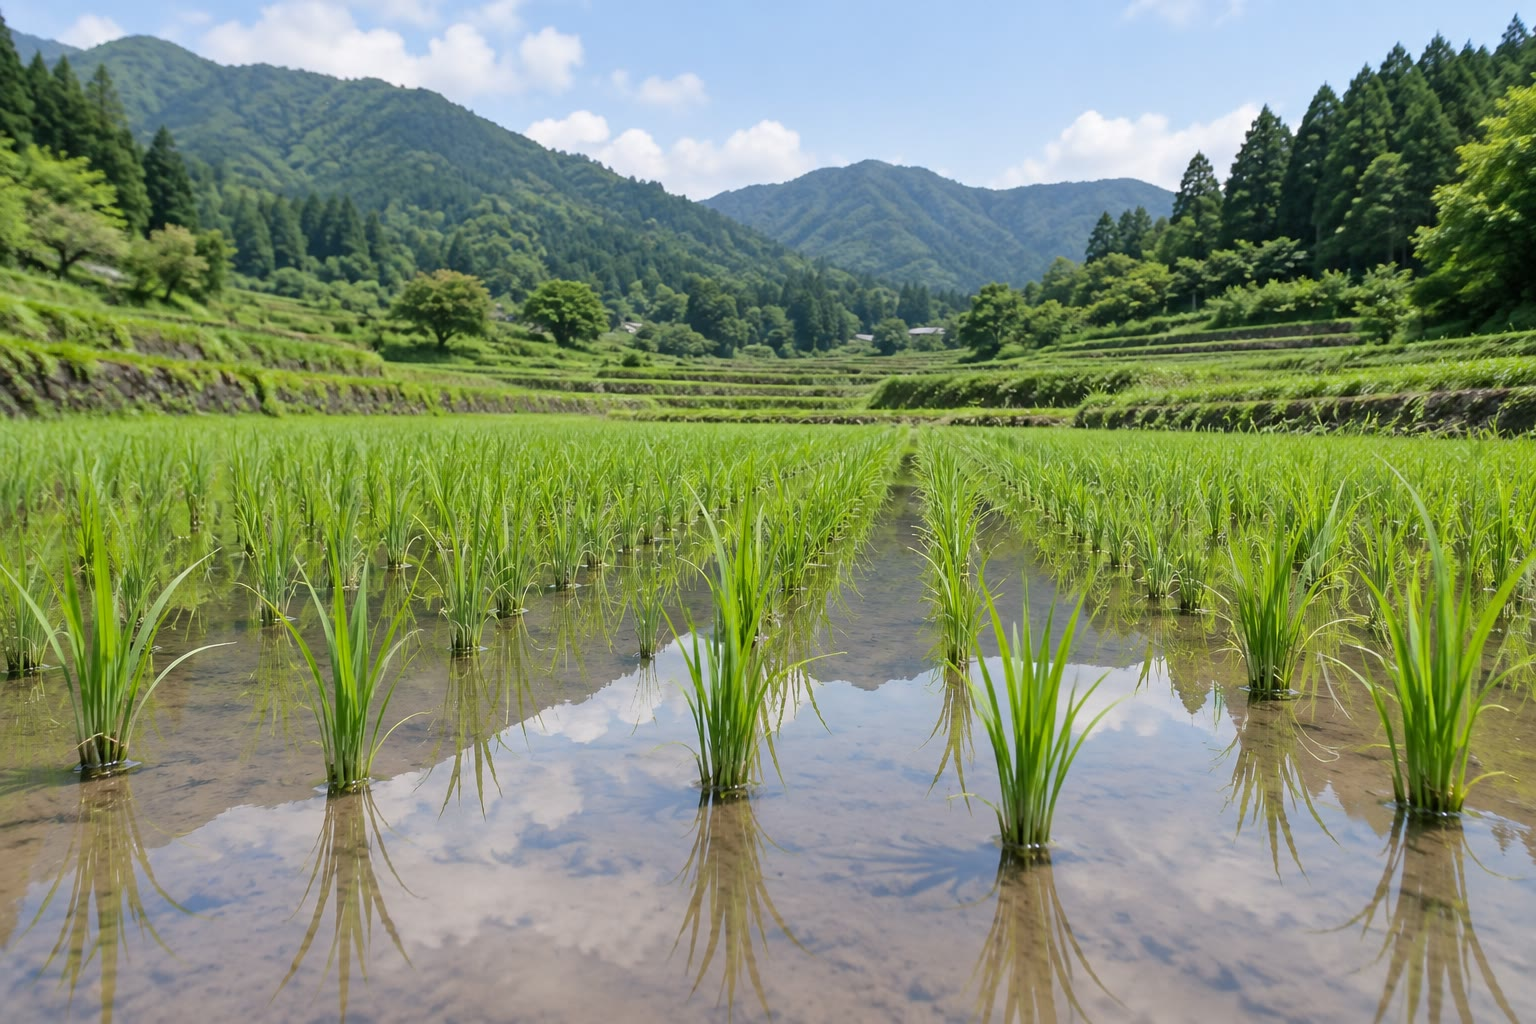
\includegraphics[width=0.44\linewidth]{images/book4/ai/b4-25-rice-paddy.jpg}

{\small \omterm{prop:b2:biogeochemical-cycles:nitrogen}{氮循环}的两扇“门”。左：豆科植物的根瘤，
每个根瘤都是一个小室，其中根瘤菌为其宿主固定氮。
右：被水淹没的稻田，表层以下缺氧，
\omterm{def:b2:microbial-metabolism:anaerobic}{反硝化作用}使氮返回大气，产甲烷菌则
生成甲烷。}
\end{omfigure}

\section{扰动的行星}

\begin{example}[数字说明了什么]\label{ex:b2:biogeochemical-cycles:numbers}
每年排放 \qty{10}{GtC}，大气留存分数为
$0.45$，则每年有 \qty{4.5}{GtC}，即 \qty{2.1}{ppm}，留在大气中
——这正是观测到的增长斜率。自 1850 年以来的累计排放约为
\qty{700}{GtC}，其中 \qty{290}{GtC} 在大气中（140~ppm），
其余则进入海洋和陆地。要使大气保持在任一水平，净排放必须降至
慢速汇——深海混合与风化作用——所能吸收的水平，
二者合计每年不足 \qty{1}{GtC}：
\emph{净零排放}并非口号，而是在 $\tau$ 很大时盒子模型的\omterm{def:b2:biogeochemical-cycles:reservoir}{稳态}条件。
对于氮而言，固定氮\omterm{def:b2:biogeochemical-cycles:reservoir}{通量}的翻倍
使河流中的硝酸盐翻了一番，
在密西西比河与波罗的海的河口形成了死区，
并使大气中的 $\mathrm{N_2O}$（一种\omterm{def:b2:biogeochemical-cycles:reservoir}{停留时间}约一个世纪的温室气体）增加了五分之一。
\Cref{ch:b2:global-change}将进一步讨论
这些变化对生物的后果。
\end{example}

\section{练习}

\begin{exercise}[$\star$]\label{exo:b2:biogeochemical-cycles:1}
定义\omterm{def:b2:biogeochemical-cycles:reservoir}{储库}、\omterm{def:b2:biogeochemical-cycles:reservoir}{通量}和\omterm{def:b2:biogeochemical-cycles:reservoir}{停留时间}，并计算碳在陆地植物
（450 GtC，光合作用每年 120 GtC）和深海
（\num{37000} GtC，每年交换约 100 GtC）中的
\omterm{def:b2:biogeochemical-cycles:reservoir}{停留时间}。
\end{exercise}

\begin{exercise}[$\star$]\label{exo:b2:biogeochemical-cycles:2}
将 \qty{2.5}{ppm} 每年换算为 GtC，并将
\qty{10}{GtC} 的排放量换算为 ppm。
\end{exercise}

\begin{exercise}[$\star$]\label{exo:b2:biogeochemical-cycles:3}
指出打开 $\mathrm{N_2}$ 的两个自然过程、
将其返回的过程，以及其间的三个氧化还原步骤，
并说明各步骤对应的负责生物。
\end{exercise}

\begin{exercise}[$\star$]\label{exo:b2:biogeochemical-cycles:4}
为什么在地质时间尺度上磷比氮更常限制生产力，
而在某一给定季节中氮比磷更常
成为限制因素？
\end{exercise}

\begin{exercise}[$\star\star$]\label{exo:b2:biogeochemical-cycles:5}
一个体积为 \qty{e7}{m^3} 的湖泊每年接纳 \qty{2}{t} 磷，
并每年更换其 \qty{20}{\%} 的水体。计算其\omterm{def:b2:biogeochemical-cycles:reservoir}{稳态}磷浓度，
以及输入开始后达到其 \qty{90}{\%} 所需的时间。
若输入减半，结果如何？
\end{exercise}

\begin{exercise}[$\star\star$]\label{exo:b2:biogeochemical-cycles:6}
根据基林数据，计算 $\mathrm{CO_2}$ 在
20 世纪 60 年代（十年间由 316 增至 \qty{325}{ppm}）和 2010 年代
（九年间由 390 增至 411）的平均增长速率，分别以 ppm 每年和 GtC 每年表示。
\end{exercise}

\begin{exercise}[$\star\star$]\label{exo:b2:biogeochemical-cycles:7}
莫纳罗亚山的季节性锯齿形曲线的振幅约为
\qty{6}{ppm}（峰到谷）。将其换算为 GtC，并与北半球陆地
的年净初级生产量相比较，后者约为
\qty{35}{GtC}。为什么锯齿形曲线要小得多？
\end{exercise}

\begin{exercise}[$\star\star$]\label{exo:b2:biogeochemical-cycles:8}
\omterm{prop:b2:biogeochemical-cycles:nitrogen}{固氮}酶每固定一个 $\mathrm{N_2}$ 消耗 16 个 ATP。对于一种豆科植物，
每公顷每年固定 \qty{200}{kg} 氮，计算固定的
$\mathrm{N_2}$ 的摩尔数和所消耗的 ATP，以及这些 ATP
所代表的葡萄糖质量（约每个葡萄糖对应 30 个 ATP）。该量占
\qty{10}{t/ha} 作物光合产物的多大比例？
\end{exercise}

\begin{exercise}[$\star\star$]\label{exo:b2:biogeochemical-cycles:9}
浮游生物以雷德菲尔德比 $\mathrm{C:N:P} = 106:16:1$ 生长。
深层海水中磷酸盐含量为 \qty{2.2}{\micro mol/kg}，
硝酸盐含量为 \qty{32}{\micro mol/kg}。当一团水体
被带至表层时，哪一种元素先被耗尽，
在其耗尽之前又能固定多少碳？
\end{exercise}

\begin{exercise}[$\star\star\star$]\label{exo:b2:biogeochemical-cycles:10}
将大气视为一个盒子，其中过剩碳 $E$ 以速率 $E/\tau$ 被汇移除，
并由排放量 $Q$ 补充。取 $\tau =
50$ 年、$Q = \qty{10}{GtC/yr}$，求\omterm{def:b2:biogeochemical-cycles:reservoir}{稳态}过剩量，
并换算为对应的 ppm 数。
解释为什么实际结果更糟。
\end{exercise}

\begin{exercise}[$\star\star\star$]\label{exo:b2:biogeochemical-cycles:11}
1963 年的核试验使大气中的 $\mathrm{{}^{14}C}$ 增加了一倍；此后过剩量
大约每 11 年减半，尽管 $\mathrm{{}^{14}C}$
的半衰期为 5730 年。解释所测量的是什么，以及
这 11 年告诉了我们关于\omterm{prop:b2:biogeochemical-cycles:carbon}{碳循环}的什么信息。
\end{exercise}

\begin{exercise}[$\star\star\star$]\label{exo:b2:biogeochemical-cycles:12}
“人类使\omterm{prop:b2:biogeochemical-cycles:nitrogen}{氮循环}翻了一番，而\omterm{prop:b2:biogeochemical-cycles:carbon}{碳循环}
只是稍加扰动。”请结合数字进行讨论：固定\omterm{def:b2:biogeochemical-cycles:reservoir}{通量}、占自然\omterm{def:b2:biogeochemical-cycles:reservoir}{通量}的比例，
以及受影响的\omterm{def:b2:biogeochemical-cycles:reservoir}{储库}。
\end{exercise}

\section{问题：一个世纪的碳收支}

\begin{problem}[{周末问题——一个世纪的排放
经过大气的箱式模型、海洋与陆地的分配，
从受肥田地到缺氧区的氮级联，
以及湖泊的磷收支，最终归结为大气留存比例、
2100 年的大气浓度以及
每公顷损失的氮量}]
\label{pb:b2:biogeochemical-cycles:1}
数据。1850 年大气浓度：\qty{285}{ppm}；\qty{1}{ppm} $=
\qty{2.13}{GtC}$。1850--2020 年的累计排放量：\qty{700}{GtC}；
2020 年大气中的 $\mathrm{CO_2}$ 浓度为 \qty{412}{ppm}。一块
\qty{1}{ha} 的田地每年施用 \qty{150}{kg} 氮肥；
作物吸收 \qty{60}{\%}，\qty{25}{\%} 发生反硝化，其余
被浸出。一座 \qty{5e7}{m^3} 的湖泊每年更新其十分之一的水体，
并每年接收 \qty{5}{t} 磷。

\medskip
\noindent\textbf{第一部分——大气留存比例。}
\begin{enumerate}
  \item 计算 1850 年和 2020 年大气中的碳量，以及
        其增加量（以 GtC 计）。
  \item 计算 1850--2020 年间的大气留存比例。
  \item 其余的碳去了哪里？给出两个碳库，并由
        命题给出它们的大致份额。
  \item 若海洋吸收了排放量的 \qty{25}{\%}，
        其溶解无机碳（\qty{38000}{GtC}）相对增加了多少？
        为什么表层海洋仍会
        出现可测量的酸化？
  \item 排放量呈指数增长时，为什么大气留存比例
        大体保持不变？（考虑\omterm{thm:b2:biogeochemical-cycles:box}{箱式模型}，
        取 $Q \propto e^{t/T}$，库项为 $E/\tau$。）
  \item 若排放量保持不变并持续许多世纪，
        大气留存比例将变为多少？
\end{enumerate}

\medskip
\noindent\textbf{第二部分——未来一个世纪。}
建立超出 1850 年水平的过剩碳 $E$ 的模型，
方程为 $\mathrm{d}E/\mathrm{d}t = Q - E/\tau$，$\tau = 100$ 年。
\begin{enumerate}[resume]
  \item 计算 2020 年的过剩量（以 GtC 计）。
  \item 令 $Q$ 保持为 \qty{10}{GtC/yr}，计算\omterm{def:b2:biogeochemical-cycles:reservoir}{稳态}
        过剩量及其所隐含的浓度。
  \item 从 2020 年起求解 $E(t)$，取 $Q = 10$，并给出
        2100 年时的 $E$ 及其对应的浓度。
  \item 现设 $Q$ 在 2020 年至 2070 年间线性降至零，
        并保持为零。计算 2070 年的 $E$（积分该方程；
        线性 $Q$ 的特解为一次式加一个
        常数），并计算 2100 年的过剩量。
  \item 比较两种情形下 2100 年的浓度。
  \item 为什么对第二种情景而言，采用单一的 $\tau$ 会过于乐观？
\end{enumerate}

\medskip
\noindent\textbf{第三部分——氮级联。}
\begin{enumerate}[resume]
  \item 计算作物吸收、反硝化和淋失的氮量，
        以每公顷每年计。
  \item 淋失的氮以硝酸盐形式进入河流，继而
        进入大海，浮游生物按雷德菲尔德比利用它。
        它能使浮游生物固定多少碳？
  \item 这些碳下沉并在深层被呼吸，同时消耗
        氧气，每个 C 消耗 1 个 $\mathrm{O_2}$。计算所消耗的氧量，
        分别以摩尔和千克表示。
  \item 饱和时，每立方米海水约含 \qty{0.25}{mol} 的
        $\mathrm{O_2}$。多少立方米的底层水，
        会因一公顷的淋失量而脱氧？
  \item 反硝化的部分以 $\mathrm{N_2O}$ 形式部分逸出，
        占反硝化氮量的 \qty{1}{\%}。计算 $\mathrm{N_2O}$
        每公顷每年的排放量，及其以 $\mathrm{CO_2}$ 计的增温当量，
        （按每千克计，$\mathrm{N_2O}$ 的增温效应是 $\mathrm{CO_2}$ 的 270 倍）。
  \item 与制造肥料时所排放的 $\mathrm{CO_2}$ 相比，
        （每千克氮按\omterm{prop:b2:biogeochemical-cycles:nitrogen}{哈伯–博施法}制取，约排放 \qty{4}{kg}
        的 $\mathrm{CO_2}$）。
\end{enumerate}

\medskip
\noindent\textbf{第四部分——湖泊。}
\begin{enumerate}[resume]
  \item 若唯一的损失途径是冲刷，计算湖泊磷的\omterm{def:b2:biogeochemical-cycles:reservoir}{停留时间}，
        以及其\omterm{def:b2:biogeochemical-cycles:reservoir}{稳态}浓度，单位为
        \unit{mg/m^3}。
  \item 磷含量超过 \qty{30}{mg/m^3} 的湖泊称为
        \omterm{prop:b2:biogeochemical-cycles:ps}{富营养化}湖泊。该湖是否属于此类？
  \item 沉积作用也会移除磷，其时间常数为
        5 年。重新计算\omterm{def:b2:biogeochemical-cycles:reservoir}{停留时间}和
        浓度。
  \item 输入量减至每年 \qty{1}{t}。计算新的
        \omterm{def:b2:biogeochemical-cycles:reservoir}{稳态}，以及进入其 \qty{10}{\%} 范围内所需的时间。
  \item 为什么许多湖泊的恢复速度比本计算
        所预测的更慢？
  \item 计算湖泊磷每年按雷德菲尔德比
        可构建进浮游生物的碳量，依据
        \qty{5}{t} 的输入量。
  \item 给出结果：大气留存比例、
        2100 年的两个浓度，以及每公顷
        淋失的氮量。
\end{enumerate}
\end{problem}
